\subsection*{Case 5} % Baseware 
\label{case: 5} 
% Inference architecture
% \begin{figure*}[t]
% \centering
% 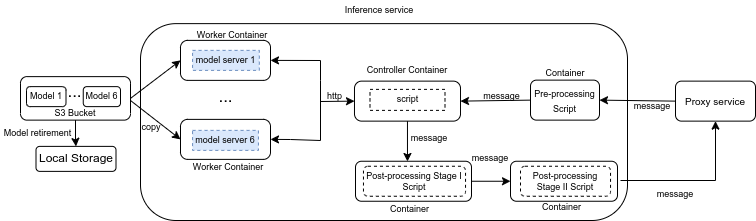
\includegraphics[width=0.8\textwidth]{images/case5_deployment_process_v2.png}
% \caption{Case 5 deployment setup}
% \label{fig: case5_deployment_process}
% \end{figure*}

% deployment setup diagram
\begin{figure*}[t]
\centering
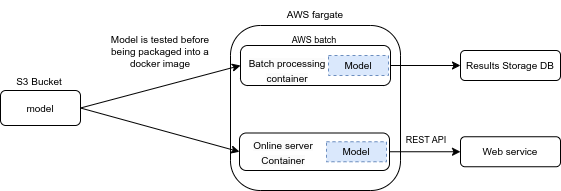
\includegraphics[width=0.8\textwidth]{images/case4_deployment_process_v2.png}
\caption{Case 4 Inference Architecture}
\label{fig: case4_deployment_process}
\end{figure*}

The case company provides electronic invoice management solutions facilitating invoice data exchange. The AI system is a part of this solution. It mainly extracts data fields from a PDF invoice and converts them into text format, which the user can submit to electronic invoice processing systems. Underlying the AI system is an optical character recognition model that uses a combination of NN techniques to extract and predict an invoice’s text field. This system levels the field for SMEs that still use PDF invoices, but the model must handle many unseen PDF layouts during inference.


\textit{Pre-Deployment}: The ML system consists of 6 models (approx. 350MB each) that provide inference concurrently, and each model is trained on a subset of the dataset. Multiple models are designed to improve confidence in the overall prediction results through a voting mechanism. One version of each model is stored in an S3 bucket where other components of the inference architecture access the model. As a retirement policy, once a model is considered for retirement from production, it is stored in an offline server while the online version is deleted from the inference server.

\textit{Quality assurance}: The deployment workflow includes a CI/CD (Bamboo) pipeline with staging and production environments in a cloud setting. The quality assurance process begins with performing local tests on each model by running inference on a dataset of around 1000 documents. These local tests serve as the acceptance tests, and models that pass these tests proceed to the staging environment, where integration and regression testing occurs. Coverage and accuracy metrics are collected at this stage to determine whether the models meet the required quality standards for moving to the production stage. Once in the production environment, an additional testing step is performed using around 20 documents to ensure the model remains functional.

\textit{Server Environment}: The model binary is packaged into a docker container where it is directly accessed during inference. The inference service contains multiple components in a micro-service architecture, including data processing containers, a controller container, and six worker containers that generate inferences. The elements communicate through a messaging queue service (AWS Messaging), but the controller container communicates with the worker containers using HTTP. The data processing and the controller docker containers run scripts (no server), but the worker nodes are Python-based server containers. The controller node distributes inference jobs to the six independent worker servers, which carry out the predictions and return results to the controller node. The architecture is generally designed as a serverless setup using scripts to perform tasks and a messaging protocol to communicate across components.

% Re-Write the inference section a bit to introduce the inference pipeline
\textit{Inference}: To perform inference, a proxy service typically submits a request to an input queue specifying the location of the documents needing processing. The system then pre-processes these documents and generates predictions on various form fields. These predictions are submitted to an output message queue in JSON format. The proxy service can retrieve the predicted results from the output queue for further use. This process is typically performed in a batch mode for more optimal inference processing.

As shown in Figure~\ref{fig: case5_deployment_process}, the inference pipeline is a modular sub-system composed of containerized scripts and a server that performs inference. This setup is optimal for scaling at the sub-process level. The first set of containers (data generators) download a document in PDF format, extract data from it, and transform the data into an array of characters per document. These obtained data objects are then packaged in JSON format and submitted to a queue where the next container in the pipeline ("the batcher") collects and batches several records, effectively processing multiple documents. The batching container stores the batch of character arrays in an S3 bucket in JSON format. 

The next component of the pipeline is a container (controller) that fetches the batched data from the S3 bucket, transforms the data into Numpy arrays, and then submits the data to the models for inference through HTTP requests. There are six models, each in a server container(worker) that produces inference and responds to the controller container when the inference has been completed. A given worker container fetches the array of characters from the S3 bucket and converts them to Numpy arrays before submitting them to the model for inference. The worker further transforms obtained predictions from Numpy arrays to JSON arrays stored in the S3 bucket. After the successful execution of the inference process, a worker reports to the controller, and the controller sends a message to a queue where the next container (extractor) in the pipeline will post-process the results.

Post-processing of the results involves conducting heuristics and local basic checks to determine the quality of inference results. At this stage, the results are also automatically or manually validated based on the threshold of defined accuracy. This process is completed by sending batch results to a message queue where the final component of the pipeline will fetch the results. %(audio segment 49:00).

The final component in the pipeline is also a containerized script that de-batches the results into independent results per document, followed by performing any necessary transformations of the results before submitting them into the final queue where the proxy service fetches results.

\textit{Monitoring}: Monitoring involves checking the system's general availability. Splunk collects logs, monitors resources, and sends alerts in case of a service outage. The coverage metric is calculated by comparing the proportion of documents with confidently accurate inference results to those requiring human validation to confirm their inference results. If the ratio of documents that need human validation increases, it can indicate a decrease in coverage and potentially degrading model performance.